\documentclass[main_tikz.tex]{subfiles}
%\usetikzlibrary{...}

%\usepackage{beamerarticle}
%\graphicspath{{../images/}}
\begin{document}

\begin{tikzpicture}
\tikzset{
    %Define standard arrow tip
    >=stealth',
    boxes/.style={
        align=left,
        rounded corners=3pt,
        draw,
        thin,
        black,
    },
    arrow/.style={
        ->, ultra thick,
        shorten <=5pt, shorten >=5pt
    },
    splitted/.style={
        rectangle split,
        rectangle split parts=2,
    },
    wdata/.style={
        text width=8em,
        align=center
    },
}


\node (origin) at (0, 0) {};

\draw[arrow] ($(origin) + (-2.5em, 0)$)
    node[boxes, left, wdata] (data) {Données\\Vectorielles}
          -- ($(origin) + (2.5em, 0)$)
    node[boxes, right, wdata] {
        \only<-2>{Classification\\ Régression\\ Prédiction}
        \only<3>{Quantification\\Résumé\\Visualisation}};
    
\draw[draw, dashed] ($(origin) + (-25em, -3.5em)$)
    node[right,align=center, fill=lightblue!70] {\bf Exemple:}
                 -- ($(origin) + (12em, -3.5em)$);

\draw[arrow] ($(origin) + (-2.5em, -10em)$)
    node[boxes, left, splitted, wdata] {
        \only<1>{Données cliniques\\d'une tumeur}
        \only<2>{Représentation\\intermédiaire}
        \only<3>{Représentation\\apprise}
        \nodepart{second} \vskip.3em
            \only<1>{Taille, Grade\\ Histologie\\ Mutation\\...}
            \only<2>{Feature\\engineering\\Apprentissage profond}
            \only<3>{\vskip1em {\Huge ?}\vskip1em}
        \vskip.1em\phantom{.}
    }
          -- ($(origin) + (2.5em, -10em)$)
    node[right, wdata] {
        \vskip.3em
            \only<1>{Réponse au\\traitement\\[1.5em]Prédiction de survie}
            \only<2>{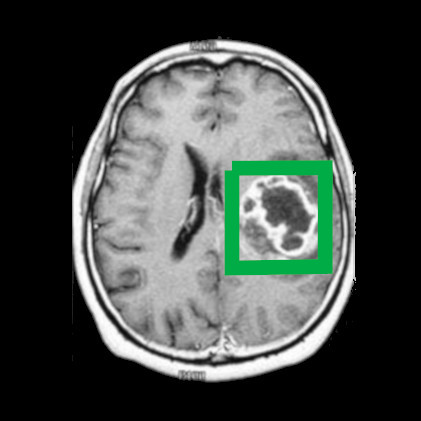
\includegraphics[width=6em]{machine_learning_for_signals/tumeur_annotated}}
         \vskip.1em\phantom{.}
    };


\node[boxes, above, left, wdata] (label) at ($(origin) + (-2.5em, 5em)$) {
    Annotation
};

\uncover<-3>{\draw[arrow, gray] (label.east) -- (origin.east) ;}
\uncover<2-3>{\draw[arrow, gray] (label.west) -- ($(data.west) + (-2.5em, 0)$);}

\uncover<2->{
\draw[arrow] ($(data.west) + (-5em, 0)$) node[boxes, left, wdata] (signal) {Signaux} -- (data.west);


%\node[left, draw, inner sep=0, splitted, wdata, rounded corners=3pt, clip] (imagenet) at ($(data.west) + (-5em, -10em)$) {
%    \only<2>{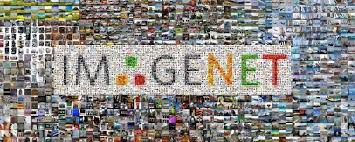
\includegraphics[height=3.5em]{machine_learning_for_signals/imagenet.jpg}}
%    \only<3>{Signaux physiologiques}
%    \nodepart{second} \vskip.3em
%       \only<2>{Taille, Grade\\ Histologie\\ Mutation\\$\cdots$}
%       \only<3>{ECG\\Radiographie\\EEG\\$\cdots$}
%    \vskip.1em\phantom{.}};

\node[left] (signals) at ($(data.west) + (-5em, -10em)$) {};

\node[left] () at ($(signals) + (-4em, 2em)$) {
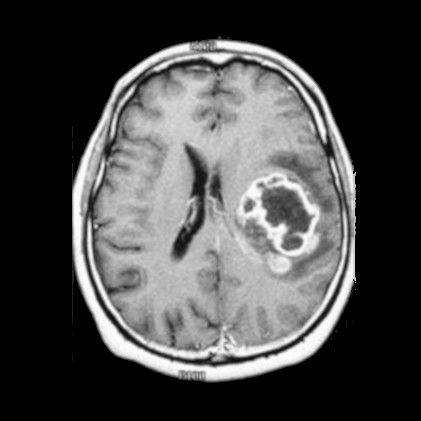
\includegraphics[width=4em]{machine_learning_for_signals/tumeur}
};
\node[left] () at ($(signals) + (.5em, 2em)$) {
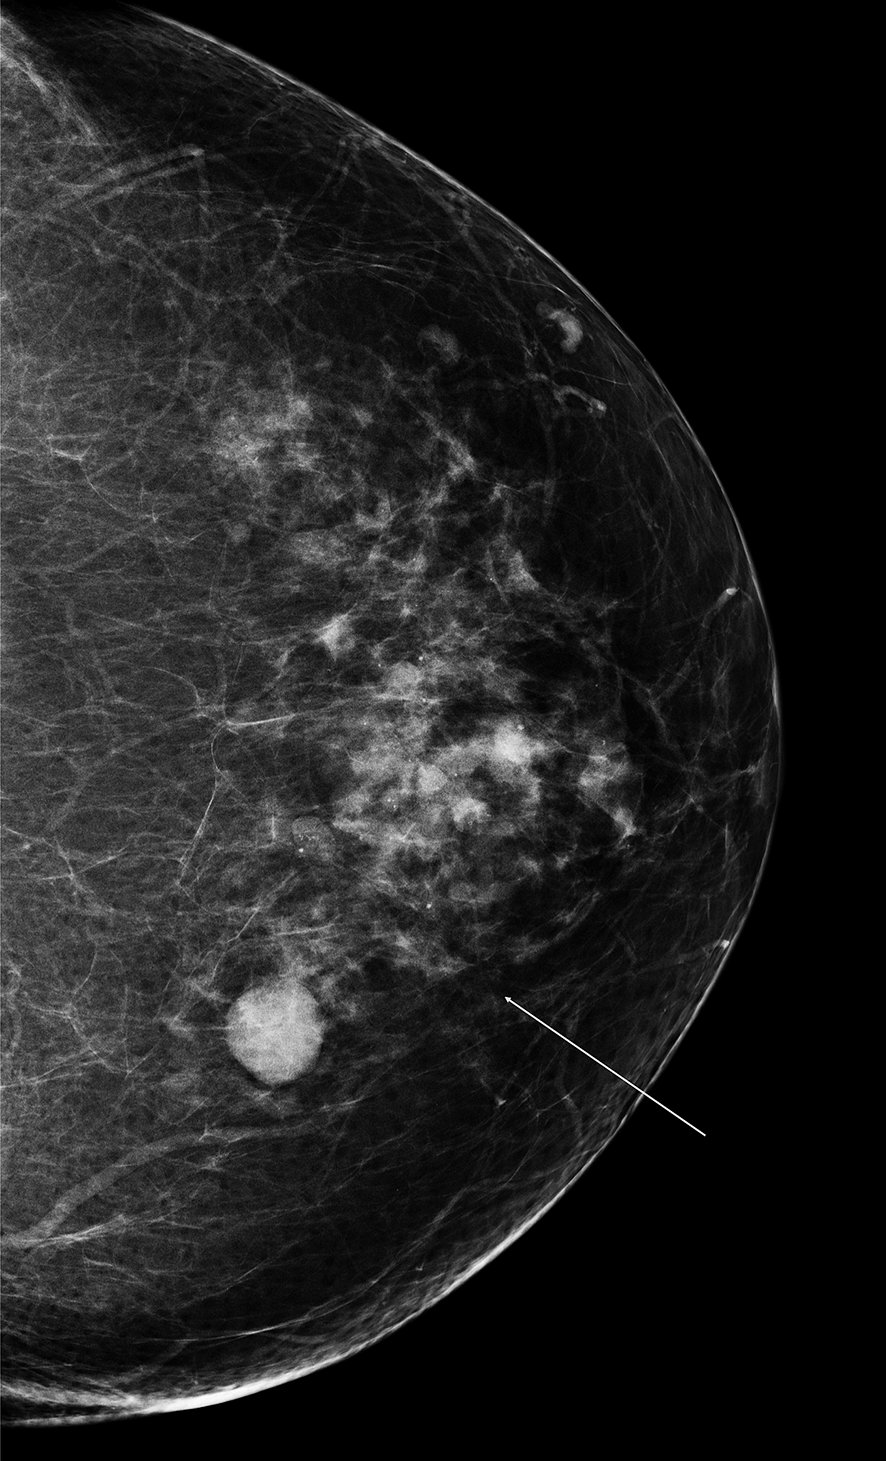
\includegraphics[width=4em]{machine_learning_for_signals/mamographie}
};
\node[left] () at ($(signals) + (-0em, -3em)$) {
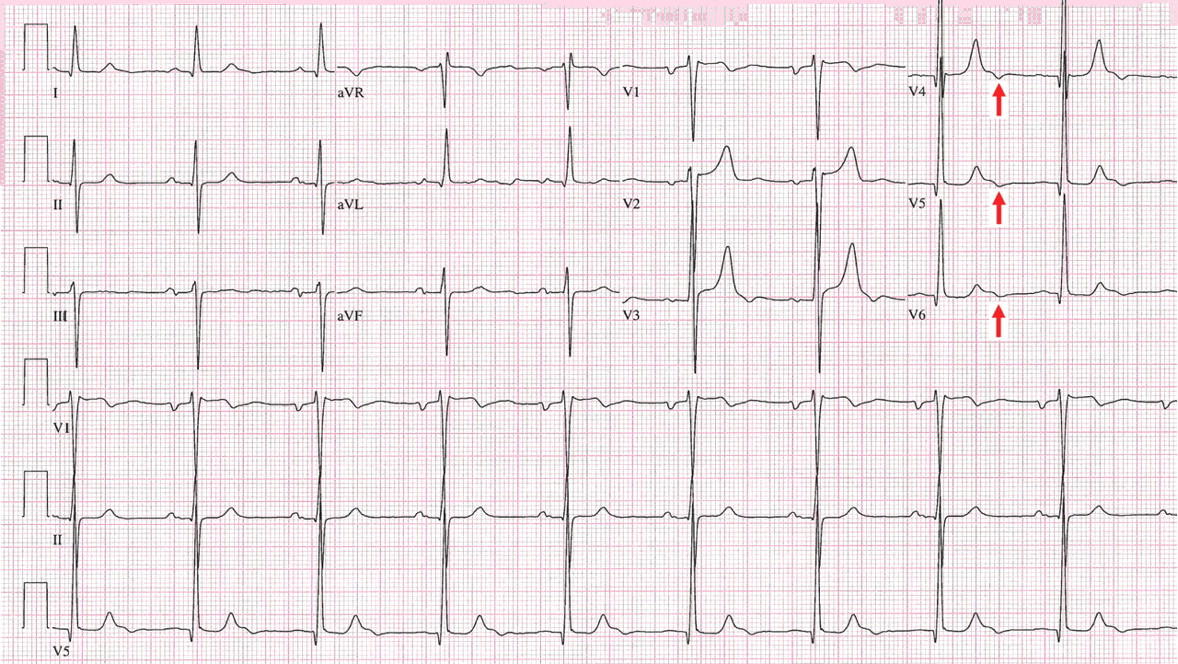
\includegraphics[width=8em]{machine_learning_for_signals/aortic_insuffisency}
};


\draw[arrow] (signals.east) --
              ($(data.west) + (0, -10em)$);

}

\uncover<4->{
    \draw[ultra thick, red] ($(label) + (2em, 1em)$) -- ($(label) - (2em, 1em)$);
    \draw[ultra thick, red] ($(label) + (2em, -1em)$) -- ($(label) - (2em, -1em)$);
}


\end{tikzpicture}


\end{document}
